\documentclass{beamer}
\mode<presentation>
\usepackage{amsmath}
\usepackage{amssymb}
%\usepackage{advdate}
\usepackage{adjustbox}
\usepackage{subcaption}
\usepackage{enumitem}
\usepackage{multicol}
\usepackage{mathtools}
\usepackage{listings}
\usepackage{url}
\usepackage{hyperref}
\def\UrlBreaks{\do\/\do-}
\usetheme{Boadilla}
\usecolortheme{lily}
\setbeamertemplate{footline}
{
  \leavevmode%
  \hbox{%
  \begin{beamercolorbox}[wd=\paperwidth,ht=2.25ex,dp=1ex,right]{author in head/foot}%
    \insertframenumber{} / \inserttotalframenumber\hspace*{2ex} 
  \end{beamercolorbox}}%
  \vskip0pt%
}
\setbeamertemplate{navigation symbols}{}

\providecommand{\nCr}[2]{\,^{#1}C_{#2}} % nCr
\providecommand{\nPr}[2]{\,^{#1}P_{#2}} % nPr
\providecommand{\mbf}{\mathbf}
\providecommand{\pr}[1]{\ensuremath{\Pr\left(#1\right)}}
\providecommand{\qfunc}[1]{\ensuremath{Q\left(#1\right)}}
\providecommand{\sbrak}[1]{\ensuremath{{}\left[#1\right]}}
\providecommand{\lsbrak}[1]{\ensuremath{{}\left[#1\right.}}
\providecommand{\rsbrak}[1]{\ensuremath{{}\left.#1\right]}}
\providecommand{\brak}[1]{\ensuremath{\left(#1\right)}}
\providecommand{\lbrak}[1]{\ensuremath{\left(#1\right.}}
\providecommand{\rbrak}[1]{\ensuremath{\left.#1\right)}}
\providecommand{\cbrak}[1]{\ensuremath{\left\{#1\right\}}}
\providecommand{\lcbrak}[1]{\ensuremath{\left\{#1\right.}}
\providecommand{\rcbrak}[1]{\ensuremath{\left.#1\right\}}}
\theoremstyle{remark}
\newtheorem{rem}{Remark}
\newcommand{\sgn}{\mathop{\mathrm{sgn}}}
\providecommand{\abs}[1]{\left\vert#1\right\vert}
\providecommand{\res}[1]{\Res\displaylimits_{#1}} 
\providecommand{\norm}[1]{\lVert#1\rVert}
\providecommand{\mtx}[1]{\mathbf{#1}}
\providecommand{\mean}[1]{E\left[ #1 \right]}
\providecommand{\fourier}{\overset{\mathcal{F}}{ \rightleftharpoons}}
%\providecommand{\hilbert}{\overset{\mathcal{H}}{ \rightleftharpoons}}
\providecommand{\system}{\overset{\mathcal{H}}{ \longleftrightarrow}}
	%\newcommand{\solution}[2]{\textbf{Solution:}{#1}}
%\newcommand{\solution}{\noindent \textbf{Solution: }}
\providecommand{\dec}[2]{\ensuremath{\overset{#1}{\underset{#2}{\gtrless}}}}
\newcommand{\myvec}[1]{\ensuremath{\begin{pmatrix}#1\end{pmatrix}}}
\let\vec\mathbf

\lstset{
%language=C,
frame=single, 
breaklines=true,
columns=fullflexible
}

\numberwithin{equation}{section}

\title{NCERT-10.4.1.2.2}
\author{Arnav Mahishi \\ Dept. of Electrical Engg.\\IIT Hyderabad.}

\date{\today} 
\begin{document}

\begin{frame}
\titlepage
\end{frame}
\section*{Outline}
\section{Problem}
\begin{frame}
\frametitle{Problem Statement}
The product of two consecutive integers is $306$. We need to find the integers.
\end{frame}
%\subsection{Literature}
\section{Solution}
\subsection{Input Parameters}
\begin{frame}
\frametitle{Input Parameters}
\begin{table}[h!]
    \centering
    \begin{tabular}[12pt]{ |c| c|}
    \hline
    \textbf{Variable} & \textbf{Description}\\ 
    \hline
         $x$& The bigger integer out of the two we need to find\\
         \hline
         $g\brak{x}$& The function we take to update $x_n$ in the point iteration method\\
         \hline
         $x_{\alpha,n}$& The value of x after n iterations for the first root\\
         \hline
          $x_{\beta,n}$& The value of x after n iterations for the second root\\
          \hline
    \end{tabular}
    \label{tab:my_label}
\end{table}
\end{frame}
\subsection{Theoritical Soln}
\begin{frame}
\frametitle{Theoritical Soln}
Lets start by assuming the bigger integer as $x$ and the smaller integer as $\frac{306}{x}$
\begin{align}
    \implies x-\frac{306}{x}=1\\
    \implies x^2-306=x\\
    \implies x^2-x-306=0
\end{align}
Using the quadratic formula:
\begin{align}
    x=\frac{1\pm\sqrt{1^2-\brak{4\cdot -306}}}{2}\\
    x_1=\frac{1+\sqrt{1225}}{2}=18\\
    x_2=\frac{1-\sqrt{1225}}{2}=-17
\end{align}
\end{frame}
\begin{frame}
If $x=18$ the other integer will be $17$ if $x=-17$ the other integer will be $-18$
\begin{align}
    p\brak{2}=41-72\brak{-2}-18\brak{-2}^2=113
\end{align}
$\therefore$ The integers can be $18,17$ or $-18,-17$\
\end{frame}
\subsection{QR algo}
\begin{frame}
    \frametitle{Qr Algorithm}
    The QR algorithm is as follows:
 QR decomposition 
\begin{align}
A = QR
\end{align}

     $Q$ is an $ m \times n $ orthogonal matrix
     $R$ is an $n \times n$ upper triangular matrix.

Given a matrix $ A = [a_1, a_2, \dots, a_n] $, where each $ a_i $ is a column vector of size $ m \times 1 $.

 Normalize the first column of $A$:
\begin{align}
q_1 = \frac{a_1}{\norm{a_1}}
\end{align}
\end{frame}
\begin{frame}
  For each subsequent column $ a_i $, subtract the projections of the previously obtained orthonormal vectors from $ a_i $ :
\begin{align}
a_i' = a_i - \sum_{k=1}^{i-1} \langle a_i, q_k \rangle q_k
\end{align}
Normalize the result to obtain the next column of \( Q \):
\begin{align}
q_i = \frac{a_i'}{\norm{a_i'}}
\end{align}

Repeat this process for all columns of \( A \).

 Finding $R$:- \\
After constructing the ortho-normal columns $ q_1, q_2, \dots, q_n $ of $Q$, we can compute the elements of $R$ by taking the dot product of the original columns of $A$ with the columns of $Q$:

\begin{align}
    r_{ij} = \langle a_j, q_i \rangle \text{ , for  }  i \leq j 
\end{align}

\end{frame}

%\section{Plot}
\subsection{Companion matrix}
\begin{frame}[fragile]
\frametitle{Companion Matrix}
For the given polynomial equation the companion matrix will be
\begin{align}
	\Lambda = \myvec{0 & 1\\306 & 1}
\end{align}
 Initialization \\
Let $A_0 = A $, where $A$ is the given matrix.
QR Decomposition \\
For each iteration $ k = 0, 1, 2, \dots $:

     Compute the QR decomposition of \( A_k \), such that:
    \begin{align}
    A_k = Q_k R_k
    \end{align}
    where:
    
         $Q_k $ is an orthogonal matrix ($ Q_k^\top Q_k = I $).
         $ R_k $ is an upper triangular matrix.
    
    The decomposition ensures $ A_k = Q_k R_k $.

     Form the next matrix \( A_{k+1} \) as:
    \begin{align}
    A_{k+1} = R_k Q_k
    \end{align}
\end{frame}
\begin{frame}
 Convergence\\
Repeat Step 2 until $ A_k $ converges to an upper triangular matrix $ T $. The diagonal entries of $T$ are the eigenvalues of $A$.\\
 The eigenvalues of matrix will be the roots of the equation. We can intorduce a shift to make the convergence faster
\begin{align}
\sigma &= 1\\
\Lambda_{\text{shifted}} &= \myvec{0 & 1\\306& 1} - \sigma I\\
\Lambda_{\text{shifted}} &= \myvec{-1 & 1\\ 306 & 0}
\end{align}
Where $\sigma$ is the last diagonal element.
\end{frame}
\begin{frame}
In our case:
\begin{align}
    \Lambda=\myvec{0&1\\306&1}\\
    \implies B=\myvec{a_{11}&a_{12}\\a_{21}&a_{22}}=\myvec{0&1\\306&1}\\
    \implies d=\frac{a_{11}-a_{22}}{2}=-0.5\\
\implies shift=a_{22}-sgn\brak{d}\sqrt{d^2+a_{12}a_{21}}=18.5\\
    \hat{A}_0=A_0-shift\cdot I=\myvec{-18.5&1\\306&-17.5}\\
    \implies Q_0=\myvec{-0.0603&0.9982\\0.9982&0.0603}\\R_0=\myvec{306.5586&-17.5285\\0&-0.0579}\\
    \implies A_1=R_0Q_0+shift\cdot I=\myvec{-17.4965&-304.9422\\-0.0578&18.4965}
\end{align}
\end{frame}
\begin{frame}
After 19 iterations the matrix converges to
\begin{align}
    A_{19}=\myvec{-17&-305\\4.97\times 10^{-11}&18}
\end{align}
The sub-diagonal elements are nearly zero confirming convergence and the diagonal elements are the eigenvalues. The eigen values given by the code are
\begin{align}
	x_1 = 18.000000000433293,
	x_2 = -17.000000000043303
\end{align}
\end{frame}
\begin{frame}[fragile]
\frametitle{Plot}
\begin{figure}[h!]
   \centering
   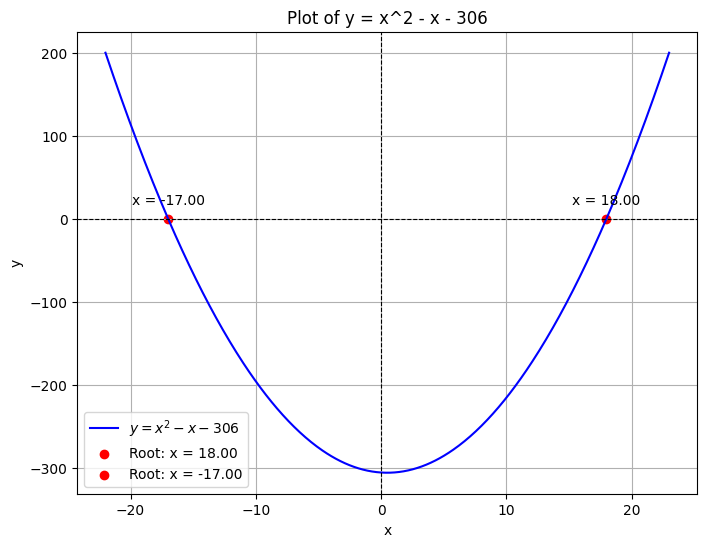
\includegraphics[width=1\linewidth]{./figs/fig.png}
   \caption{Comparison between the Theoretical solution and Computational solution}
   \label{stemplot}
\end{figure}
\end{frame}
\end{document}
